\documentclass[letter, 10pt]{article}
\usepackage[utf8]{inputenc}
\usepackage[spanish, es-tabla]{babel}
\usepackage{amsfonts}
\usepackage{amsmath}
\usepackage[dvips]{graphicx}
\usepackage{graphicx}
\usepackage{subfigure} % subfiguras
\DeclareGraphicsExtensions{.bmp,.png,.pdf,.jpg}
\usepackage{xcolor,listings}%color support for listings
\usepackage{epstopdf}
\usepackage{algpseudocode}
\usepackage{algorithm}
\usepackage{url}
\usepackage{caption}
\usepackage[justification=centering]{caption}
\usepackage{cite}
\usepackage[top=3cm,bottom=3cm,left=3.5cm,right=3.5cm,footskip=1.5cm,headheight=1.5cm,headsep=.5cm,textheight=3cm]{geometry}



\begin{document}



\title{Análisis Inteligente de Datos \\ \begin{Large}Tarea 3\end{Large}}
\author{Paulina Aguila - Felipe Flores}
\date{14 de julio de 2016}

\maketitle


\begin{figure}[ht]
\begin{center}

\includegraphics[width=0.2\textwidth]{Images/Isotipo-Negro.png}\\
\end{center}
\end{figure}
\vspace{2cm}

\section{Reducción de Dimensionalidad para Clasificación}

La reducción de dimensionalidad es un proceso que tiene mucha importancia dentro del análisis de datos, ya que ayuda a la visualización y la exploración de los datos, también reduce el costo computacional del procesamiento de los datos debido a que son menos dimensiones. Otro beneficio importante de la reducción de dimensionalidad, es que reduce significativamente el riesgo de \textit{overfitting} o sobre ajuste del modelo.\\

En esta primera sección, se trabajará con datos sobre sonidos fonéticos que debe ser identificados con vocales del inglés británico. Los datos se representan en un espacio de 10 características ($d=10$), en donde 528 registros corresponden a datos de entrenamiento y 462 son datos de prueba. Los autores reportan que el mejor desempeño corresponde a un 56\% de accuracy y se alcanza con un modelo de vecinos más cercanos y una red neuronal artificial de radio basal.\\

A través del lenguaje de programación Python, se cargan los datos de la fuente \cite{D1} y se llevan a un dataframe de entrenamiento con 528 registros y un dataframe de prueba con 462 registros.\\

Para cada conjunto de datos (entrenamiento y test), se deben normalizar los datos. Este es un paso muy importante, ya que permite ajustar la escala de las variables a la varianza de la unidad, lo que hace que los valores de datos que se encuentran ubicados en los extremos, no ejerzan un peso excesivo en la función objetivo.\\

Utilizando PCA (Análisis de Componentes Principales) se genera una representación en dos dimensiones para el dataset inicial (10 dimensiones). La Figura \ref{G1.1}, muestra la clasificación que realiza PCA.

\begin{figure}[h]
\begin{center}
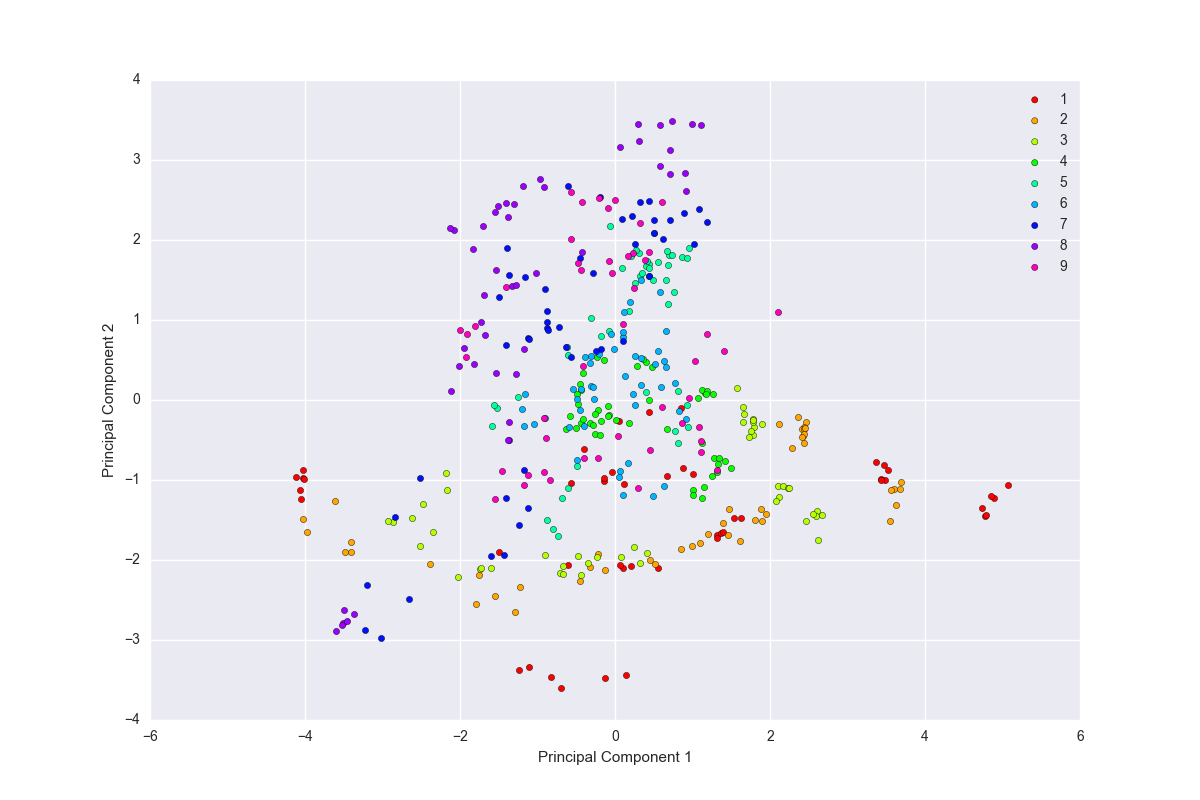
\includegraphics[width=1\textwidth]{Images/figure_1.png}
\caption{Gráfica que muestra las dos componentes principales de PCA diferenciando con distintos colores las 9 clases.}
\label{G1.1}
\end{center}
\end{figure}

Utilizando LDA (Linear Discriminant Analysis) se genera una representación en dos dimensiones para el dataset inicial (10 dimensiones). La Figura \ref{G1.2}, muestra la clasificación que realiza LDA.\\

\begin{figure}[h]
\begin{center}
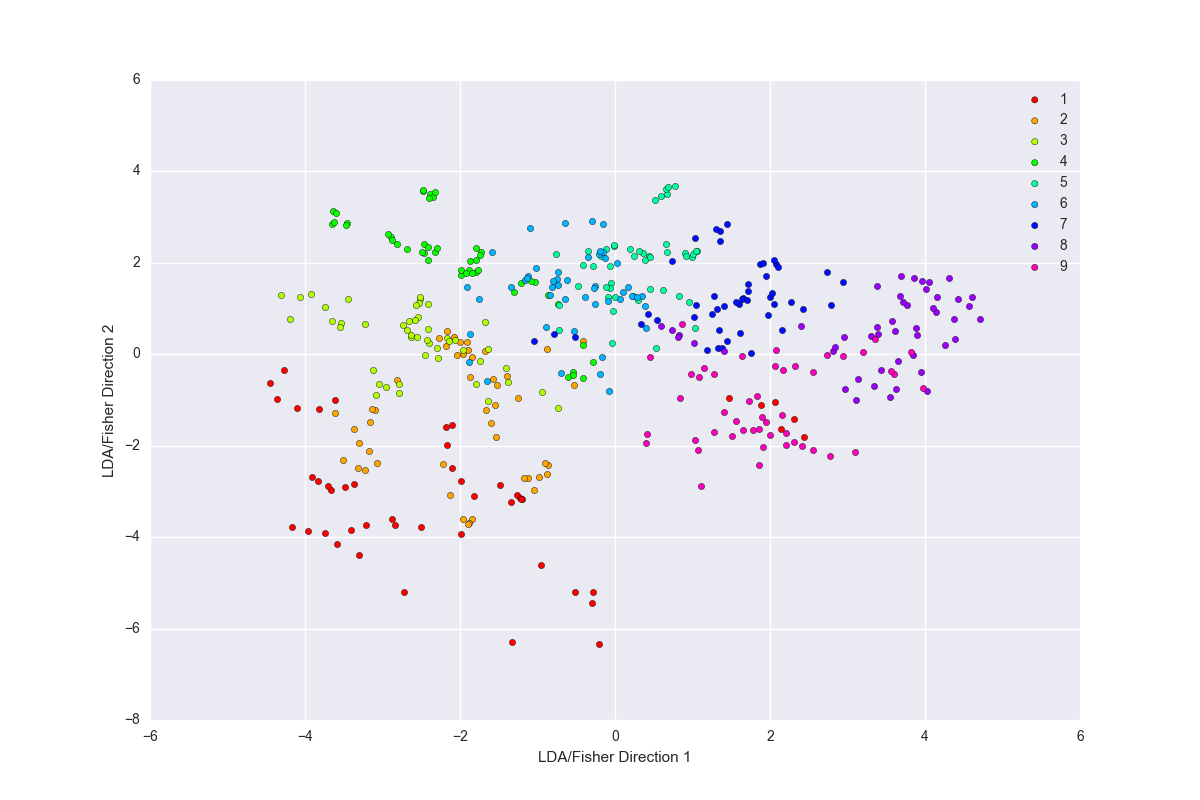
\includegraphics[width=1\textwidth]{Images/figure_2.png}
\caption{Gráfica que muestra las dos componentes principales de LDA diferenciando con distintos colores las 9 clases.}
\label{G1.2}
\end{center}
\end{figure}

Al analizar las Figuras \ref{G1.1} y \ref{G1.2}, se puede observar que en ambas se redujo la dimensionalidad de 10 a 2 componentes. Sin embargo, con PCA se observa que las clases no están separadas lo suficiente como para diferenciarlas, pero al utilizar LDA, se puede ver que las clases se separan más entre sí. Esto se puede deber a que LDA es un método de clasificación que en este caso se utiliza para reducir dimensionalidad y evitar el \textit{overfitting}.\\

Para el caso de querer clasificar un registro $x$ escogido aleatóriamente considerando solo la probabilidad a priori de cada clase, se debe calcular la probabilidad de ocurrencia de cada clase, luego en base a la ecuación (1), se selecciona la clase que tiene mayor probabilidad.

\begin{equation}
j=\underset{i}{Argmax} (P(y=C_i))
\end{equation}

En el siguiente ítem, se utilizaron los métodos de clasificación LDA, QDA y KNN, sin realizar reducción de dimensionalidad. A continuación, la Tabla \ref{table:score} muestra un resumen con los valores del accuracy para cada uno de estos modelos tanto con los datos de entrenamiento como con los de test.

\begin{table}[!hbt] 
\begin{center}
\begin{tabular}{| l | c | c | c |} 
\hline
\textbf{} & \textbf{LDA} & \textbf{QDA} &\textbf{KNN (k=10)} \\ 
\hline 
Train set & 0.6837 & \textbf{0.9886} & 0.9318\\ 
Test set &0.4524 & 0.4156 & \textbf{0.4913}\\
\hline 
\end{tabular}
\caption{Recuadro con el score o accuracy para cada método aplicado a datos de entrenamiento o de prueba.} 
\label{table:score}
\end{center} 
\end{table}

De la Tabla \ref{table:score}, se puede ver que para el conjunto de datos de train el método que mejor se comporta es QDA, mientras que al aplicarlo a los datos de test el método KNN tiene la mejor accuracy.\\

La Figura \ref{G1.3} que se muestra a continuación, muestra un gráfico en donde se aplica el método KNN variando el valor de k desde 1 a 10, con respecto al score o accuracy. Se puede apreciar que cuando k=7 entonces el método KNN funciona mejor y tiene mejor score.\\

\begin{figure}[h]
\begin{center}
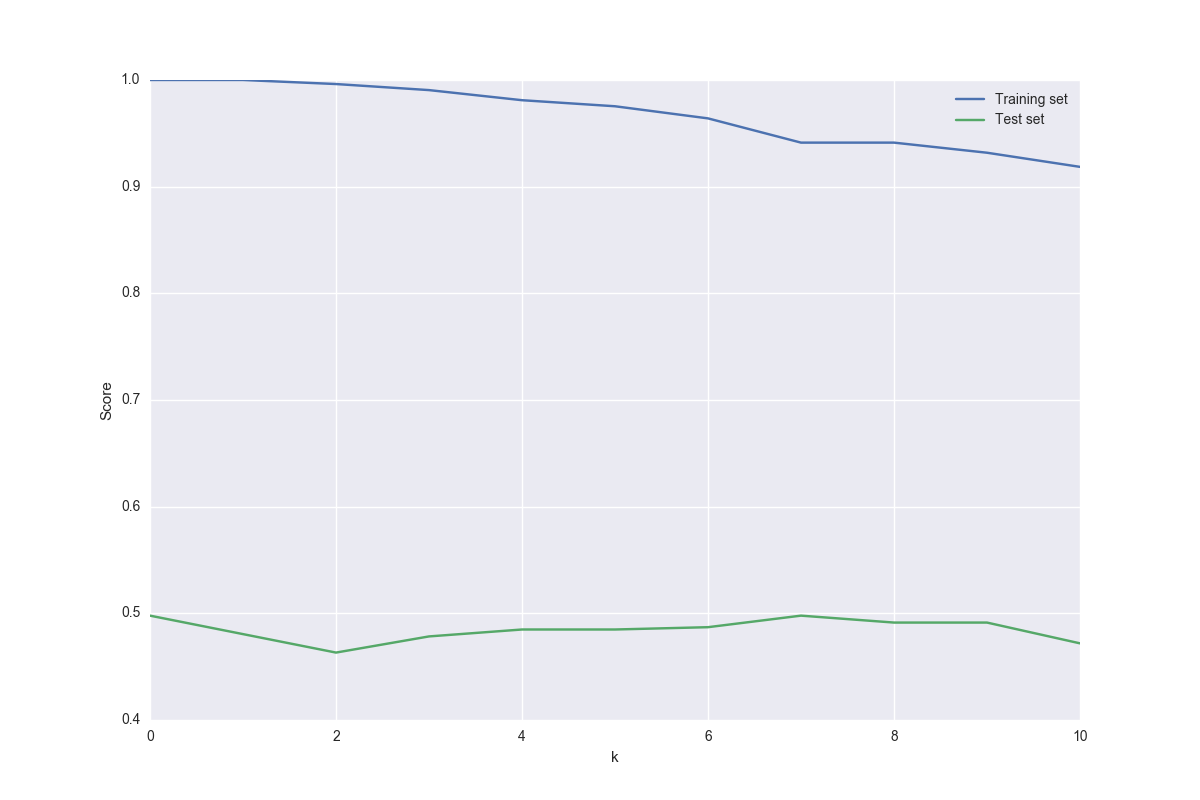
\includegraphics[width=0.8\textwidth]{Images/figure_3.png}
\caption{Gráfica que muestra las dos componentes principales de LDA diferenciando con distintos colores las 9 clases.}
\label{G1.3}
\end{center}
\end{figure}

Para la última parte, se realizó reducción de domiensionalidad con los métodos PCA y LDA, para cada uno de los cuales se fue variando la cantidad de dimensiones desde 1 hasta la máxima 10, además, para cada iteración se clasificó el modelo con LDA, QDA y KNN (k=7), calculando los errores de clasificación para los datos de entrenamiento y para los de test. Estos errores se graficaron obteniéndose los gráficos de las Figuras \ref{pca} y \ref{lda}.\\

\begin{figure}[h]
\begin{center}
\subfigure[LDA]{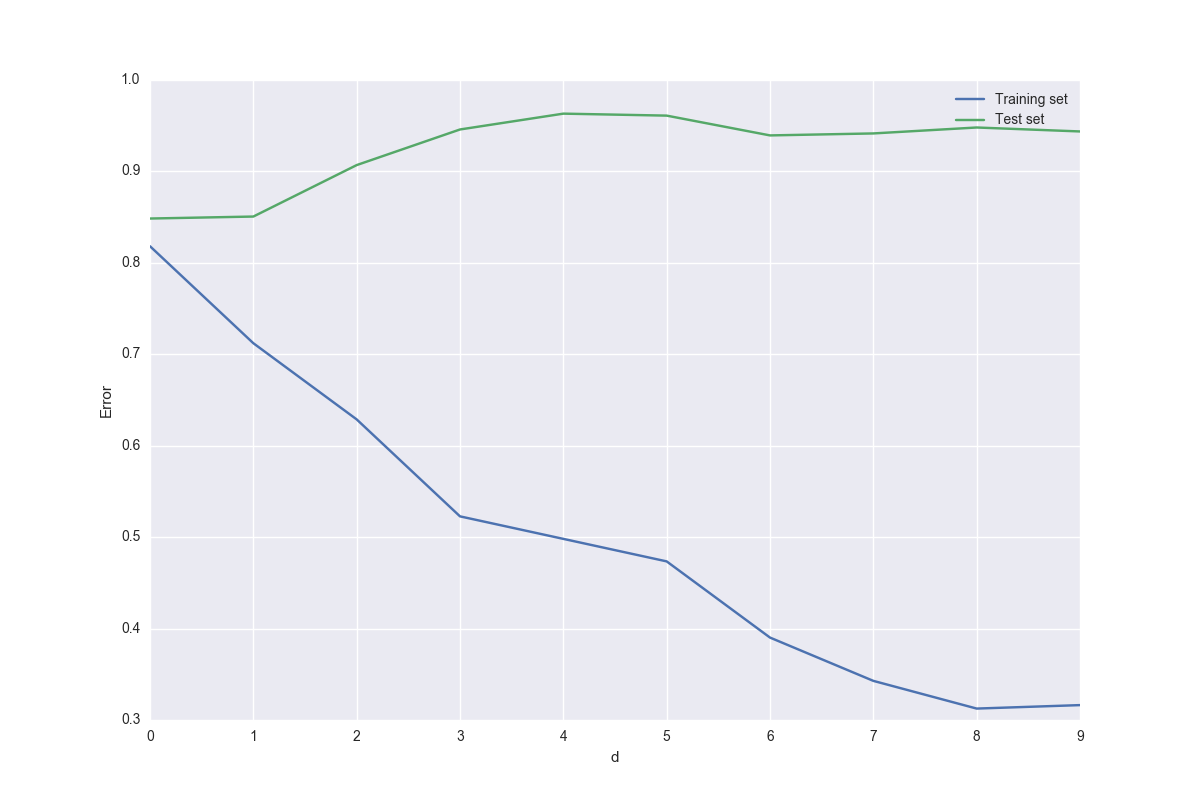
\includegraphics[width=0.6\textwidth]{Images/figure_4.png}}
\subfigure[QDA]{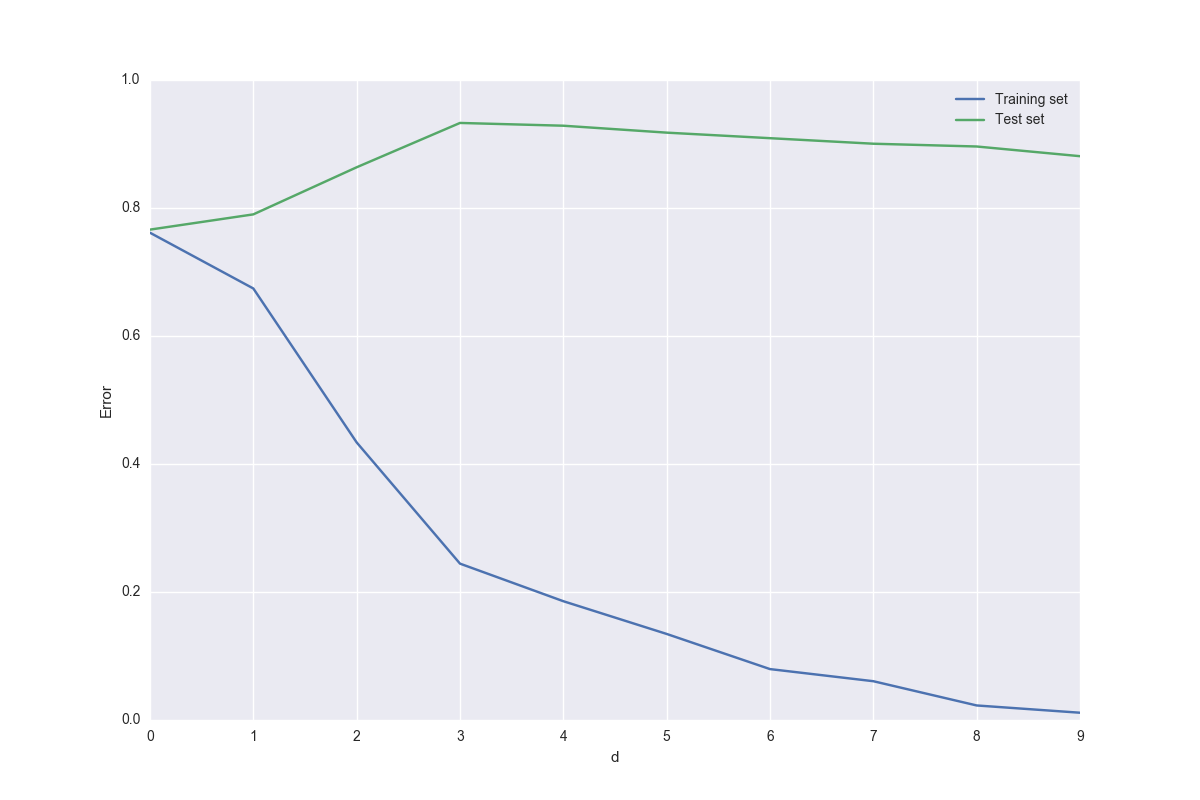
\includegraphics[width=0.6\textwidth]{Images/figure_5.png}}
\subfigure[KNN (k=7)]{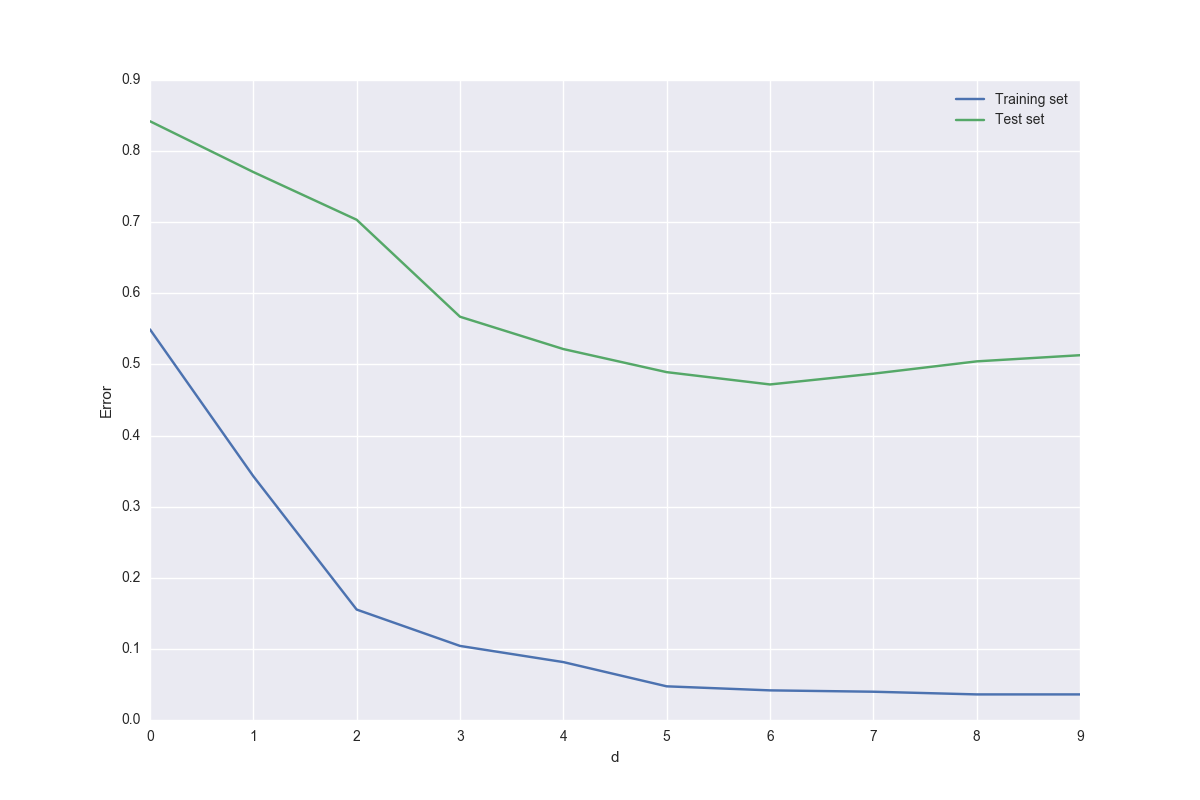
\includegraphics[width=0.6\textwidth]{Images/figure_6.png}}
\caption{Gráficas de los errores de clasificación haciendo reducción de dimensionalidad con PCA con d dimensiones.} 
\label{pca}
\end{center}
\end{figure}

Para la Figura \ref{pca}, se puede ver que la cantidad de dimensiones igual a 7 es óptima ya que reduce el error de clasificación para los datos de test, comportándose de mejor manera el método LDA. Para la Figura \ref{lda}, se observa que con una cantidad de dimensiones igual a 2 se tiene un menor error para los datos de prueba, siendo el más estable LDA no variando mucho su error al aumentar de dimensionalidad.\\

\begin{figure}[h]
\begin{center}
\subfigure[LDA]{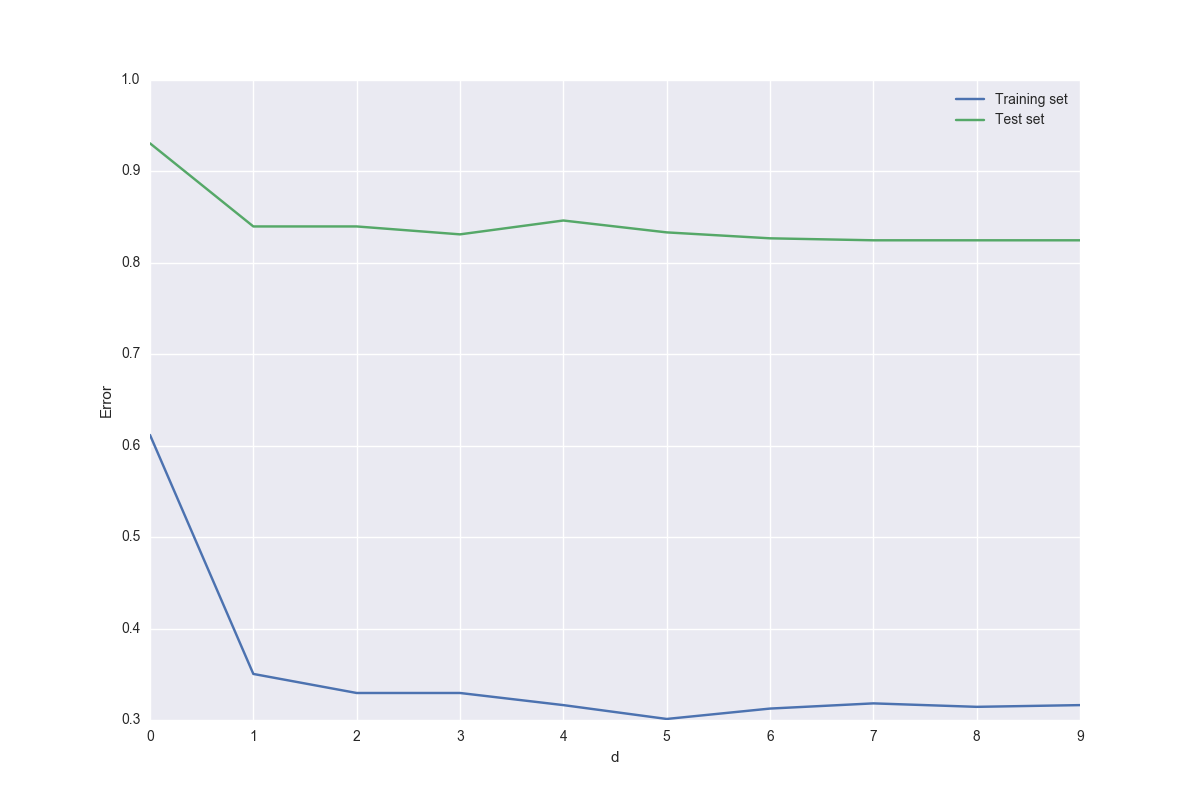
\includegraphics[width=0.6\textwidth]{Images/figure_7.png}}
\subfigure[QDA]{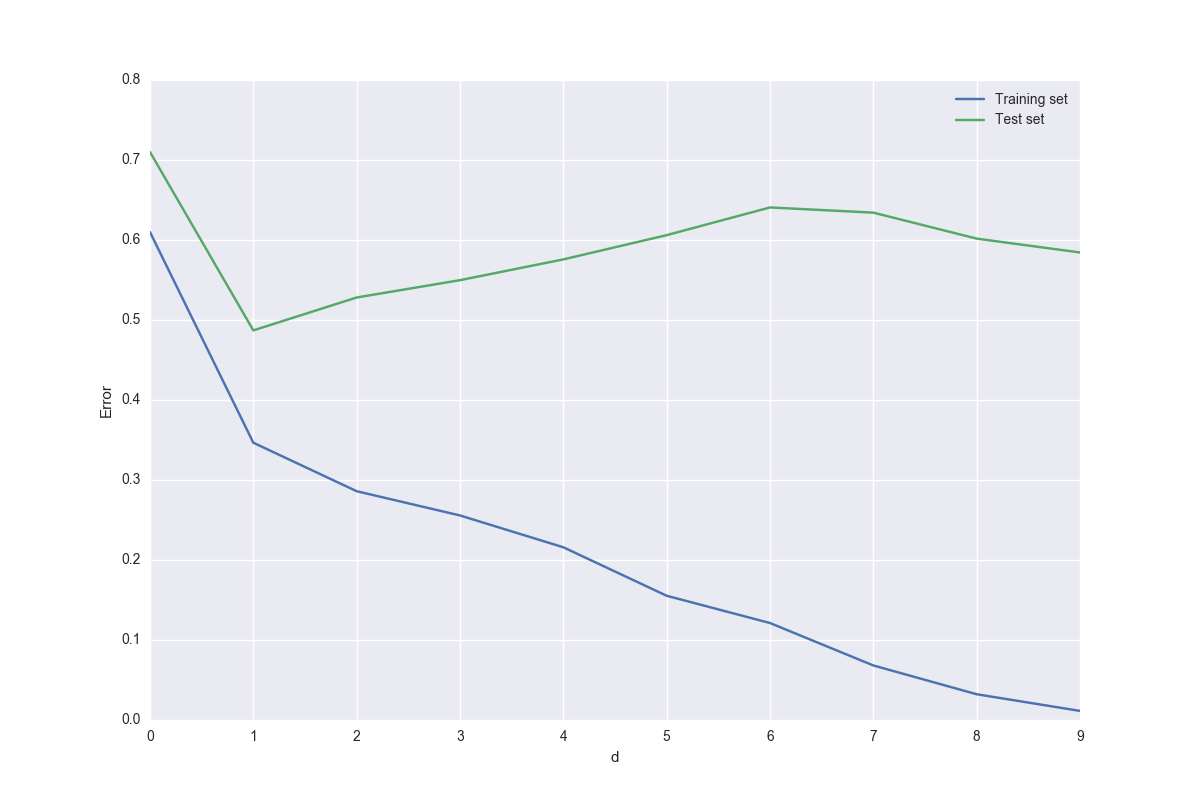
\includegraphics[width=0.6\textwidth]{Images/figure_8.png}}
\subfigure[KNN (k=7)]{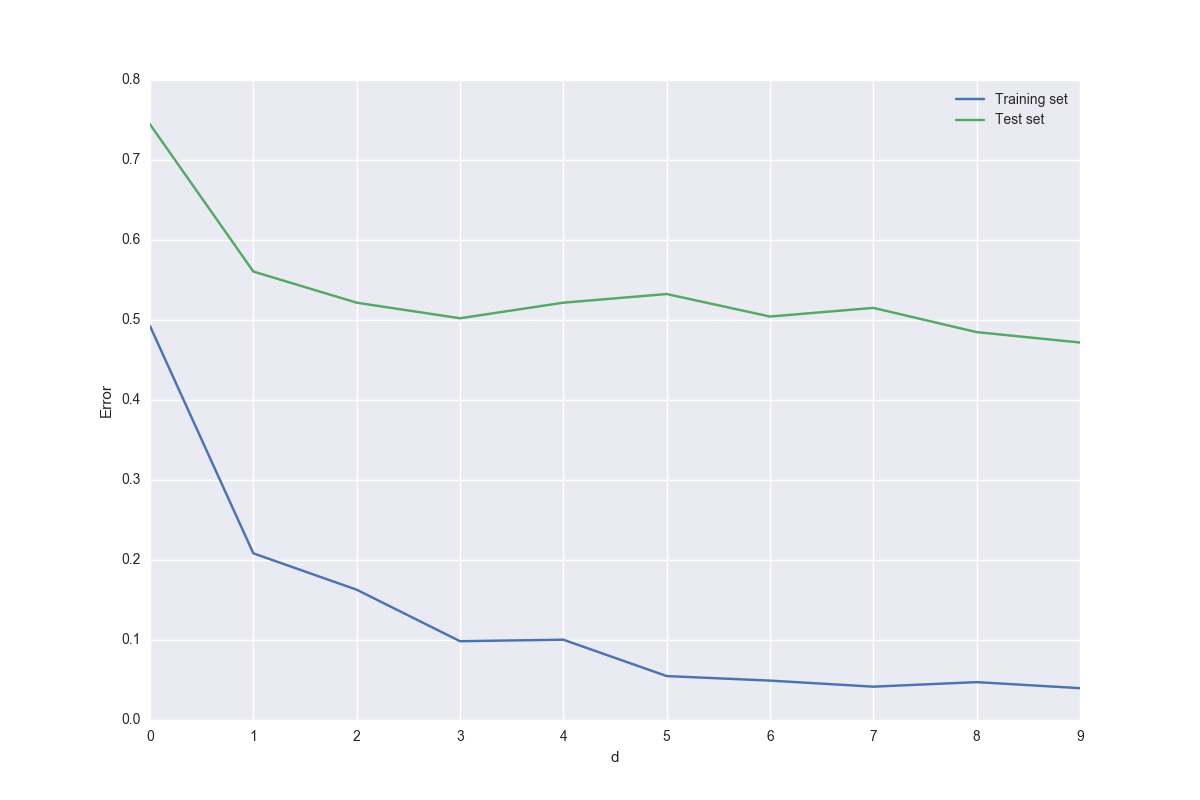
\includegraphics[width=0.6\textwidth]{Images/figure_9.png}}
\caption{Gráficas de los errores de clasificación haciendo reducción de dimensionalidad con LDA con d dimensiones.} 
\label{lda}
\end{center}
\end{figure}

\section{Análisis de Opiniones sobre Películas}

En esta sección se realiza análisis de sentimiento sobre películas de una Dataset publicado en Kaggle. El dataset es una colección de opiniones de películas etiquetadas con +1 y 0 si la opinión es positiva o negativa respectivamente. 
Datos de Entrenamiento: 3554 registros.
Datos de Test: 3554 registros.
El dataset tiene 2 dimensiones.
El conjunto de datos tiene 2 clases.
De la data de entrenamiento 1784 registros tienen una opinión negativa y 1770 opinión positiva. En el caso de la data de test, 1803 son opiniones positivas y 1751 opiniones negativas. El dataset es tratado convirtiendo todo el texto a minúsculas, eliminando signos de puntuación y palabras sin significado como artículos, pronombres y proposiciones. Además existen dos técnicas que permiten convertir las palabras a su tronco léxico, la lematización y el stemming, técnicas similares, pero con diferentes resultados, a continuación se muestran ejemplos donde se usan ambas técnicas sobre ciertos textos, para poder entender la diferencia entre ambas.\\

Stemming		/	sin tratamiento		/	lematice:\\
love eat cake		/	I love to eat cake		/	love eat cake\\
love eat cake		/	I love eating cake		/ 	love eating cake\\
love eat cake		/	I loved eating the cake	/	loved eating cake\\
love eat cake		/	I do not love eating cake	/ 	love eating cake\\
n't love eat cake	/	I don't love eating cake	/ 	n't love eating cake\\\\
Luego se cortan las frases y se realiza un conteo de las palabras contenidas, al ver que palabras son las más recurrentes para los diccionarios formados para el set de entrenamiento y el de prueba:
Para el set de entrenamiento se tienen: charact, comedi, director, doe, even, feel, film, get, good, ha, hi, like, look, make, movi, much, one, perform, stori, thi, time, way, well, work.\\

Para el set de prueba: charact, comedi, director, doe, even, film, good, ha, hi, like, make, movi, much, one, perform, stori, thi, time, well, work.\\

Luego se realiza análisis de los resultados entregados por cuatro clasificadores distintos, con sus respectivos accuracy:\\
Clasificador Bayesiano Ingenuo Binario:
\begin{itemize}
  \item Stemming: Training accuracy=0.942881; Test accuracy= 0.747819
  \item Lematización: Training accuracy=0.877603; Test accuracy=0.681677
\end{itemize}


Clasificador Bayesiano Multinomial:
\begin{itemize}
  \item Stemming: Training accuracy=0.942319; Test accuracy=0.749789
  \item Lematización: Training accuracy=0.879291; Test accuracy=0.685055
\end{itemize}


Regresión Logística Regularizada:
\begin{itemize}
  \item Stemming: 
  \begin{itemize}
    \item C=0.01: Training accuracy= 0.782217; Test accuracy=0.690684
    \item C=0.1: Training accuracy=0.880135; Test accuracy=0.731213
    \item C=10: Training accuracy=0.999719; Test accuracy=0.725303
    \item C=100: Training accuracy=1; Test accuracy=0.719111
    \item C=1000: Training accuracy=1; Test accuracy=0.711793
  \end{itemize}
  \item Lematización: 
    \begin{itemize}
    \item C=0.01: Training accuracy=0.720597; Test accuracy=0.638615
    \item C=0.1: Training accuracy=0.806978; Test accuracy=0.666479
    \item C=10: Training accuracy=0.964547; Test accuracy=0.649310
    \item C=100: Training accuracy=0.984806; Test accuracy=0.623980
    \item C=1000: Training accuracy=0.989589; Test accuracy=0.614692
  \end{itemize}
\end{itemize}

SVM
\begin{itemize}
  \item Stemming: 
  \begin{itemize}
    \item C=0.01: Training accuracy=0.873382; Test accuracy=0.729243
    \item C=0.1: Training accuracy=0.981992; Test accuracy=0.731213
    \item C=10: Training accuracy=1; Test accuracy=0.701942
    \item C=100: Training accuracy=1; Test accuracy=0.700535
    \item C=1000: Training accuracy=1; Test accuracy=0.700535
  \end{itemize}
  \item Lematización: 
    \begin{itemize}
    \item C=0.01: Training accuracy=0.801913; Test accuracy=0.663946
    \item C=0.1: Training accuracy=0.907991; Test accuracy=0.666198
    \item C=10: Training accuracy=0.984524; Test accuracy=0.610751
    \item C=100: Training accuracy=0.987057; Test accuracy=0.606248
    \item C=1000: Training accuracy=0.983118; Test accuracy=0.603152
  \end{itemize}
\end{itemize}

\begin{figure}[h]
\begin{center}
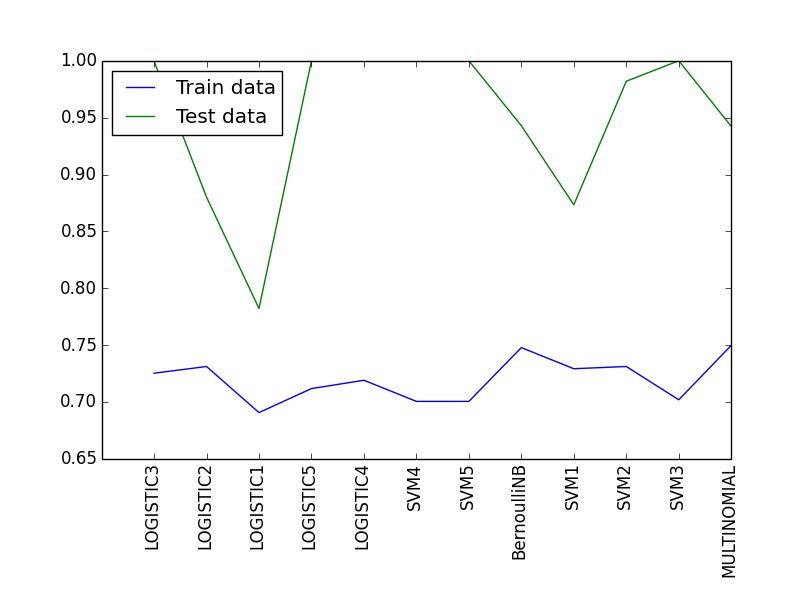
\includegraphics[width=1\textwidth]{Images/figure_pregunta_2.png}
\caption{Gráfica de accuracy de distintos clasificadores para data de test y de entrenamiento, con data preprocesada con técnica stemming.}
\label{G1.1}
\end{center}
\end{figure}

\begin{figure}[h]
\begin{center}
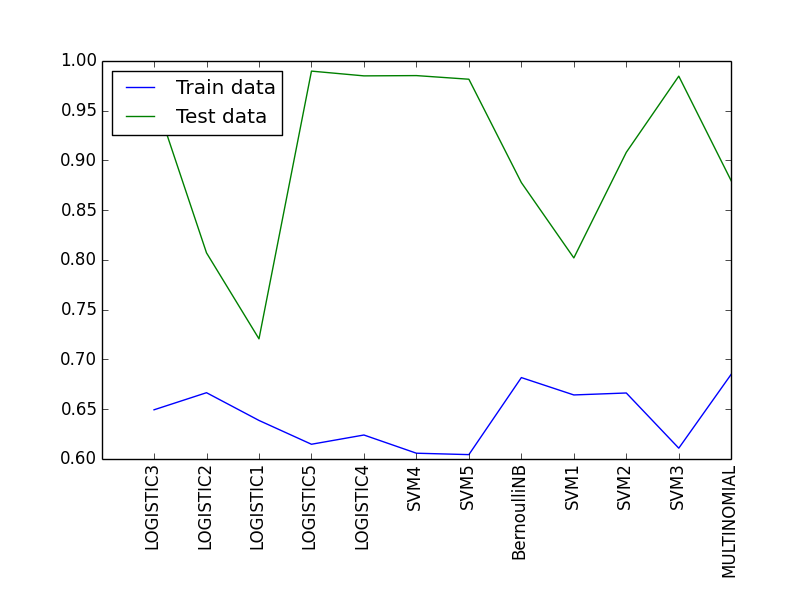
\includegraphics[width=1\textwidth]{Images/figure_pregunta2_2.png}
\caption{Gráfica de accuracy de distintos clasificadores para data de test y de entrenamiento, con data preprocesada con técnica lematización.}
\label{G1.1}
\end{center}
\end{figure}

Claramente, se aprecia que sin importar el clasificador utilizado, para nuestro dataset, los mejores resultados se obtienen preprocesando la data con la técnica de stemming, además, se tiene que los clasificadores que arrojaron mejores resultados son los Bayesianos, obteniéndose resultados muy similares entre ambos clasificadores (Multinomial y Binario). Adempas cabe destacar que al usar StopWords, se elimanron palabras claves como Not, las cuales cambian completamente el sentido de una opinión. \\
A continuación, se muestran textos aleatorios de la data de prueba para ambos métodos Bayesianos, y la probabilidad de que sea una opinión negativa o positiva respectivamente:\\
\begin{itemize}
  \item Clasificador Bayesiano Ingenuo Binario:
  \begin{itemize}
    \item  {[0.98958049  0.01041951]} each scene wreaks of routine ; the film never manages to generate a single threat of suspense .
    \item {[ 0.9561989  0.0438011]} the sort of movie that gives tastelessness a bad rap .
    \item {[ 0.81647136  0.18352864]} i don't feel the least bit ashamed in admitting that my enjoyment came at the expense of seeing justice served , even if it's a dish that's best served cold .
    \item {[ 0.1751346  0.8248654]} the film can depress you about life itself .
  \end{itemize}
  \item Clasificador Bayesiano Multinomial:
  \begin{itemize}
    \item {[ 0.29397133  0.70602867]} this mistaken-identity picture is so film-culture referential that the final product is a ghost .
    \item {[ 0.6821908  0.3178092]} . . . standard guns versus martial arts cliche with little new added .
    \item {[ 0.50196961  0.49803039]} priggish , lethargically paced parable of renewal .
    \item {[ 0.64955789  0.35044211]} brainy , artistic and muted , almost to the point of suffocation .
  \end{itemize}


\end{itemize}


Los resultados son bastante buenos, pero claramente, es difícil determinar cuando una persona utiliza sarcasmo, o la neutralidad de una opinión, por lo que quizás sería bueno probar no solo con positivo y negativo, si no que generar un rango más amplio de opiniones, agregando al menos la clase neutra. 


\end{document} 
